\chapter{Numerical applications}

\epigraph{The most obvious characteristic of science is its application: the fact that, as a consequence of science, one has a power to do things. And the effect this power has had need hardly be mentioned. The whole industrial revolution would almost have been impossible without the development of science.}{\textit{Richard Feynman \\ The Meaning of It All: Thoughts of a Citizen-Scientist}}
\minitoc

\lettrine{\color{theme}{T}}he proposed finite element discretization can be employed for different numerical applications. The chapter is organized as follows:
\begin{itemize}
	\item a boundary stabilization problem for the Kirchhoff plate and for the irrotational shallow water equations is presented in Sec. \secref{sec:bd_stab};
	\item Sec. \secref{sec:mixbd_enfor} presents a comparison of the Lagrange multiplier \ref{sec:lagrMul} and the virtual domain decomposition method \ref{sec:vdd} for the enforcement of mixed boundary conditions;
	\item a thermoelastic problem for which an analytic solution is avaiable is illustrated in Sec. \secref{sec:thelas_wave}.
\end{itemize}



\section{Boundary stabilization}\label{sec:bd_stab}

In this section, we consider the boundary stabilization of a cantilever Kirchhoff plate of the irrotational shallow water equations. For pHs a simple proportional gain assures asymptotic system of the system thanks to the LaSalle’ invariance principle \cite[chapter
6, proposition 6.2]{duindam2009}. This can be used to achieve stabilization of the undeformed configuration of the Kirchhoff plate


\subsection{Cantilever Kirchhoff plate}

\begin{figure}[t]
	\centering
	\includegraphics[width=0.5\textwidth]{part_3/applications/plate_controlled.eps}
	\caption{Cantilever plate subjected to a control forces on the lateral sides.}
	\label{fig:plate_controlled}
\end{figure}

Consider the problem (illustrated in Fig. \ref{fig:plate_controlled})
\begin{equation*}\small
\begin{bmatrix}
\rho h & 0 \\ 0 & \bm{\mathcal{C}_b} \\
\end{bmatrix}
\diffp{}{t}
\begin{bmatrix}
e_w \\ \bm{E}_\kappa \\
\end{bmatrix} = 
\begin{bmatrix}
0 & -\div\Div \\ \Hess & 0 \\
\end{bmatrix}
\begin{bmatrix}
e_w \\ \bm{E}_\kappa \\
\end{bmatrix} \qquad (x, y) \in \Omega = [0, 1]\times[0,1]
\end{equation*}
subjected to the following Dirichlet homogeneous conditions
\begin{align*}
\begin{aligned}
\partial_t e_w|_{\Gamma_D} &= 0, \\
\partial_x e_w|_{\Gamma_D} &= 0, \\
\end{aligned} \qquad {\Gamma_D} &= \left\{x = 0 \right\},
\end{align*}
and Neumann boundary control
\begin{align*}
\begin{aligned}
\widetilde{q}_n|_{\Gamma_N} &= u_F,\\
\bm{E}_\kappa \cddot (\bm{n}\otimes \bm{n})|_{\Gamma_N} &= u_M, \; \\
\end{aligned} \qquad {\Gamma_N} &= \left\{y = 0 \cup x=1 \cup y=1 \right\}.
\end{align*}
The initial conditions (compatible with the constraints) are given by
\[
e_w(x,y,0) = x^2; \qquad \bm{E}_\kappa(x,y,0) ={0}.
\]
The discretization is performed as in \eqref{eq:pHsys_findim_kirchh_hess} using the BellDG3 element \eqref{eq:BellDG3}. The Dirichlet conditions are imposed weakly using Lagrange multipliers (cf. \eqref{eq:pHsys_infdim_mult1}), that are discretized using Lagrange polynomials of order 1. The resulting system read

\begin{equation}
\begin{aligned}
\mathrm{Diag}
\begin{bmatrix}
\mathbf{M}_{\rho h}\\
\mathbf{M}_{\bm{\mathcal{C}}_b}\\
\mathbf{0}\\
\end{bmatrix}
\begin{pmatrix}
\dot{\mathbf{e}}_{w} \\
\dot{\mathbf{e}}_{\kappa} \\
\dot{\bm{\lambda}}_{\Gamma_D} \\
\end{pmatrix}
&= \begin{bmatrix}
\mathbf{0} & - \mathbf{D}_{\Hess}^\top & \mathbf{B}_{\Gamma_D}\\
\mathbf{D}_{\Hess} & \mathbf{0} & \mathbf{0} \\
-\mathbf{B}_{w, \Gamma_D}^\top & \mathbf{0} & \mathbf{0} \\
\end{bmatrix} 
\begin{pmatrix}
\dot{\mathbf{e}}_{w} \\
\dot{\mathbf{e}}_{\kappa} \\
\dot{\bm{\lambda}}_{w} \\
\dot{\bm{\lambda}}_{\partial_{\bm{n} w}} \\
\end{pmatrix} + 
\begin{bmatrix}
\mathbf{0} & \mathbf{B}_{\Gamma_N} \\
\mathbf{0} & \mathbf{0} \\
\mathbf{M}_{\partial, 1} & \mathbf{0} \\
\end{bmatrix}
\begin{bmatrix}
\mathbf{u}_{\partial, 1} \\
\mathbf{u}_{\partial, 2} \\
\end{bmatrix}, \\
\begin{bmatrix}
\mathbf{M}_{\partial, 1} & \mathbf{0} \\
\mathbf{0} & \mathbf{M}_{\partial, 2} \\
\end{bmatrix}
\begin{pmatrix}
\mathbf{y}_{\partial, 1} \\
\mathbf{y}_{\partial, 2} \\
\end{pmatrix}
&= \begin{bmatrix}
\mathbf{0} & \mathbf{0} & \mathbf{M}_{\partial, 1} \\
\mathbf{B}_{1, \Gamma_2}^\top & \mathbf{0} & \mathbf{0} \\
\end{bmatrix}\begin{pmatrix}
\mathbf{e}_{1} \\
\mathbf{e}_{2} \\
{\bm{\lambda}}_{\partial, 1} \\
\end{pmatrix}.
\end{aligned}
\end{equation}
 Starting from system \eqref{eq:discr_pl}, consider the following static control law
\begin{equation}
\bm{u} = -\bm{K} \bm{y}.
\end{equation}
System \eqref{eq:discr_pl} now reads
\begin{equation}
\begin{bmatrix}
\bm{M}_{\text{pl}} & \bm{0} \\
\bm{0} & \bm{0} \\
\end{bmatrix}\frac{\d}{\d t}
\begin{pmatrix}
\bm{e}_{\text{pl}}\\
\bm{\lambda}_D \\
\end{pmatrix}
= \begin{bmatrix}
\bm{J}_d - \bm{R} & \bm{G}_D \\
-\bm{G}_D^T & \bm{0} \\
\end{bmatrix}
\begin{pmatrix}
\bm{e}_{\text{pl}}\\
\bm{\lambda}_D \\
\end{pmatrix}.
\end{equation}
The matrix $\bm{R} = \bm{B}_N \bm{Z} \bm{B}_N^T \succcurlyeq 0$ is semi-positive definitive because of the collocated input-output feature of pH systems. The energy rate evaluates to (\cite{beattie2018linear} theorem 13)
\[\dot{H} _{\text{pl}} = - \bm{e}_{\text{pl}}^T \; \bm{R} \; \bm{e}_{\text{pl}} \le 0. \]
Therefore, the Hamiltonian energy is a Lyapunov function and the asymptotic stability of configuration $\bm{e}_{\text{pl}} = \bm{0}$ is deduced using LaSalle' invariance  principle (\cite{bookPHs}  chapter 6, proposition 6.2). As a numerical illustration a cantilever square plate clamped in $x=0$ with parameters given in Table~\ref{tab:par} is considered. The controller gain matrix is set to $\bm{K} = 100 \ \bm{I}$. The initial condition, that must be compatible with the constraints, reads $e_w(x,y,0) = x^2, \; \bm{E}_{\kappa}(x,y,0)=0$. The control law is activated after 1 second. The discrete Hamiltonian, computed using \eqref{eq:H_discr} goes almost to zero in 4 seconds (Fig. \ref{fig:H_Damped}). 

\section{Mixed boundary conditions enforcement}\label{sec:mixbd_enfor}

\subsection{Trajectory tracking of a thin beam}

\subsection{Vibroacoustic under mixed boundary conditions}

\section{Thermoelastic wave propagation}\label{sec:thelas_wave}

\section{Modal analysis of plates}